\subsection{Fornitura}
    \subsubsection{Descrizione}
     Il processo di fornitura ha lo scopo di determinare l'insieme delle attività e compiti necessari allo svolgimento del progetto. 
     In questa sezione vengono esposte le regole che i membri del team \Gruppo{} si impegnano a rispettare nel corso delle fasi di progettazione, sviluppo e consegna della piattaforma \NomeProgetto{}, per diventare fornitori nei confronti del Proponente \Proponente{}\ped{\textit{G}} e dei Committenti\ped{\textit{G}} \TV{} e \RC{}. \\
     Le attività di cui questo processo è composto, descritte poi nel dettaglio, sono:
     \begin{itemize}
        	\item{avvio;}
        	\item{preparazione della proposta;}
        	\item{contrattazione;}
        	\item{pianificazione;}
        	\item{esecuzione e controllo;}
        	\item{revisione e valutazione;}
        	\item{consegna e completamento.}
     \end{itemize}
     L'obiettivo del gruppo è quello di mantenere un costante dialogo con il Proponente\ped{\textit{G}} al fine di:
     \begin{itemize}
	\item{instaurare un rapporto di collaborazione;} 
	\item{comprenderne a fondo le richieste;}
	\item{determinare vincoli sui processi e sui requisiti;}
	\item{stimare i costi;}
	\item{promuovere una verifica continua;}
	\item{avere un riscontro efficace sul lavoro svolto.}
     \end{itemize}
    
    \subsubsection{Attività}
    \subsubsubsection{Avvio}
    Durante quest'attività, il gruppo conduce un'accurata analisi e valutazione dei requisiti presenti nelle varie proposte di capitolato\ped{\textit{G}}, sotto coordinazione del Responsabile di progetto. Tale valutazione culmina con l'accettazione o meno di ogni singola proposta.
    \subsubsubsection*{Studio di Fattibilità}
    Lo \SdF{} viene redatto dagli Analisti ed indica il risultato dell'attività di valutazione di ogni capitolato\ped{\textit{G}} proposto. Tra le informazioni da esso fornite, sono presenti:
    \begin{itemize}
        \item{\textbf{Informazioni generali}: presentano il nome del progetto, del Proponente\ped{\textit{G}} e del Committente\ped{\textit{G}};}
        \item{\textbf{Descrizione}: descrive sinteticamente il capitolato\ped{\textit{G}} sotto analisi;}
        \item{\textbf{Obiettivo finale}: rappresenta il prodotto\ped{\textit{G}} risultante dal completamento del progetto, con soddisfacimento dei requisiti;}
        \item{\textbf{Tecnologie coinvolte}: descrive le tecnologie necessarie al raggiungimento dell'obiettivo finale;}
        \item{\textbf{Aspetti positivi}: espongono gli elementi del capitolato\ped{\textit{G}} che hanno suscitato entusiasmo nel team;}
        \item{\textbf{Criticità}: analizza i punti critici ed i fattori di rischio relativi alla realizzazione del progetto;}
        \item{\textbf{Esito}: illustra la posizione finale del team nei confronti del capitolato\ped{\textit{G}}.}
    \end{itemize}
    \subsubsubsection{Preparazione della proposta}
    Il gruppo definisce ed appronta una proposta, da consegnare in risposta alle richieste del Proponente\ped{\textit{G}}.
    \subsubsubsection{Contrattazione}
    Il gruppo entra in contatto con il Committente\ped{\textit{G}}, per negoziare ed infine stipulare il contratto di fornitura del prodotto software.
    \subsubsubsection{Pianificazione}
    Il gruppo conduce una revisione dei requisiti di acquisizione, andando poi a definire un piano di gestione del progetto, in grado di garantire la qualità del prodotto software che si va a concretizzare.
    \subsubsubsection*{Piano di Progetto}
    Il Responsabile di Progetto, con l'aiuto degli Amministratori, redige un \PdP{} volto a pianificare le attività del team. Tale documento contiene:
    \begin{itemize}
       		\item{\textbf{analisi dei rischi}: viene effettuata un'approfondita attività di analisi dei fattori di rischio e vengono approntate eventuali procedure attraverso cui limitare la loro occorrenza ed i loro effetti.
       		Le valutazioni effettuate vertono principalmente verso la probabilità che un rischio si verifichi e l'entità di danno in grado di provocare;}
       		\item{\textbf{modello di sviluppo}: a seguito delle opportune valutazioni, viene scelto un modello di sviluppo da utilizzare e seguire, per la pianificazione e lo svolgimento del progetto;}
       		\item{\textbf{pianificazione}: in funzione del modello di sviluppo scelto, si effettua una pianificazione quanto più dettagliata possibile delle attività da eseguire nelle diverse fasi del progetto, stabilendo preventivamente opportune scadenze temporali e tenendo giusta considerazione degli obiettivi di qualità;}
       		\item{\textbf{preventivo}: sulla base delle attività pianificate e della loro redistribuzione ai vari ruoli di progetto, viene data una stima della quantità di lavoro necessaria per ogni fase. In funzione di tale stima viene stilata una proposta di preventivo per il costo totale del progetto, da presentare a Proponente\ped{\textit{G}} e Committente\ped{\textit{G}};}
       		\item{\textbf{consultivo}: vengono rendicontate le spese, totali e per ruolo, sostenute all'interno di ciascuna fase e data una valutazione dell'andamento rispetto a quanto era stato preventivato.}
    \end{itemize}
    
    \subsubsubsection*{Piano di Qualifica}
    I Progettisti ed i Verificatori redigono il \PdQ{}, il cui scopo è raccogliere le metriche e le strategie impiegate per garantire la qualità sia dei processi attuati che del prodotto\ped{\textit{G}}, nel tempo. Tale documento contiene:
    \begin{itemize}
       		\item{\textbf{qualità di processo}: vengono individuati processi utili allo svolgimento del progetto a partire dagli standard, vengono identificati degli obiettivi funzionali e di qualità, ed infine stabilite procedure di controllo a garanzia del raggiungimento di tali obiettivi, in funzione delle risorse disponibili;}
       		\item{\textbf{qualità di prodotto}: vengono identificate le caratteristiche principali, necessarie affinché il prodotto\ped{\textit{G}} soddisfi i requisiti previsti. Vengono poi stabilite procedure e metriche di controllo, in grado di garantire l'ottenimento di tali caratteristiche e verificarne la qualità;}
       		\item{\textbf{specifiche dei test}: devono essere definiti nel dettaglio dei test utili al collaudo del prodotto, e metodologie da implementare per garantire il loro corretto svolgimento;}
       		\item{\textbf{standard di qualità}: una volta scelti adeguati standard di qualità, questi vengono presentati e descritti;}
       		\item{\textbf{valutazioni per il miglioramento}: vengono riportate eventuali problematiche riscontrate nello svolgimento di una determinata attività o nel ricoprire uno specifico ruolo, corredate dalla relativa soluzione;}
       		\item{\textbf{resoconto delle attività di verifica}: i risultati delle attività di verifica, eseguite con riferimento alle metriche previste, devono essere inseriti in un report. Tale documentazione viene poi fornita ai soggetti interessati ed eventualmente al Proponente\ped{\textit{G}}, qualora sia coinvolto nell'attività.}
    \end{itemize}   
    \subsubsubsection{Esecuzione e controllo}
    Il gruppo implementa il piano di gestione del progetto stilato durante la fase di pianificazione, e procede con lo sviluppo del prodotto\ped{\textit{G}} software. Durante il ciclo di vita di tale prodotto\ped{\textit{G}} è fondamentale monitorare e controllare iterativamente il progresso del progetto, nonché il livello di qualità.
    \subsubsubsection{Revisione e valutazione}
    È compito del fornitore condurre iterativamente procedure di verifica e validazione del software prodotto, qualora possibile anche in collaborazione con il Proponente\ped{\textit{G}}, allo scopo di dimostrare il soddisfacimento dei requisiti concordati.
    \subsubsubsection{Consegna e completamento}
    Il gruppo consegna il prodotto\ped{\textit{G}} software completato e fornisce eventuale servizio di supporto, come specificato dal contratto.
    \subsubsection{Strumenti}
    Di seguito vengono elencati gli strumenti usati durante il processo di fornitura.
    \subsubsubsection{Microsoft Excel}
    Software per la creazione e la gestione di fogli elettronici, distribuito da Microsoft come parte della suite Microsoft Office. Utilizzato per funzioni di calcolo, produzione di tabelle, grafica e diagrammi. \\
    \begin{figure}[h!]
       	\centering
       	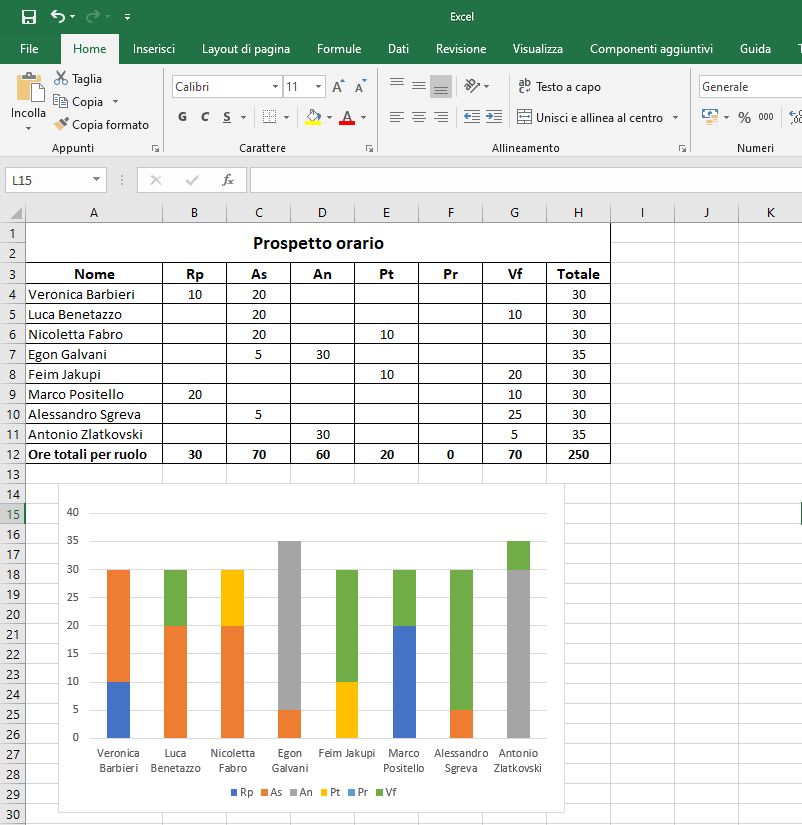
\includegraphics[scale=0.62]{./res/img/excel.png}
       	\caption{Microsoft Excel}
   	\end{figure}
    